\chapter{Sběrnicový systém KNX}
Existuje velké množství sběrnicových systémů, ale asociace KNX s 500 členskými společnostmi a 8000 produkty je v této době největší na trhu. \cite{Asociace KNX}

Pro vstup do asociace~je nutné aby žadatel splňoval požadovanou kvalitu (kompatibilita s ISO 9001~- zavedený systém kontroly kvality v podniku), vzájemná kompatibilita výrobků s ostatními členy, konfigurační kompatibilita (možná konfigurace za použití KNX Engineering Tool Software, zkráceně ETS), zpětná kompatibilita (kompatibilita starých instalací s nynějšími a budoucími instalacemi). \cite{KNX principles}

Výhodou takto velké asociace je již zmíněná vzájemná kompatibilita komponent členských společností, tisíce KNX certifikovaných skupin výrobků (pokrytí jakéhokoliv myslitelného pole aplikací), podpora všech komunikačních médií (kroucený pár TP, powerline PL, radiofrekvenční RF a rozhraní IP/Ethernet/WLAN), použití jednoho softwaru~(ETS) na projektování a programování všech výrobků členských společností. \cite{KNX principles}

KNX je také normalizováno v Evropě, USA, Číně a mezinárodně prostřednictvím norem. Tyto normy zajišťují snadné rozšíření a výměnu instalace za novou a již zmíněnou kompatibilitu mezi společnostmi. \cite{KNX basics}

\section{Historie}
\subsection{EIBA}
Asociace byla založena v Belgii, roku 1990 pod názvem European Installation Bus Association~(EIBA) se záměrem vytvářet instalace schopné komunikace pomocí sběrnic. Jako první komunikační médium byl použitý TP a aby se zajistila kompatibilita mezi produkty se členské společnosti dohodly na používání jednoho systému (standardu). Mezi další důležité milníky patří \cite{KNX history}:
\begin{itemize}
\item 1991 - první školení EIBA
\item 1992 - první certifikované zařízení na trhu
\item 1993 - představení první verze ETS na trhu 
\item 1994 - vznikl prvních školících center
\item 1996 - vznik The Scientific Partnership (spolupráce s výzkumnými institucemi)
\item[] \hspace{0.821cm} - použití PL jako komunikační médium
\end{itemize}

\subsection{KNX}
Roku 1999 se EIBA sloučila se společností Batibus Club International (BCI) a European Home Systems Association (EHSA) a~přijaly název Konnex Association. Sídlem asociace byl ustanoven Brusel. Toto sloučení nemělo vliv na zpětnou kompatibilu a~tudíž jsou všechny nové produkty kompatibilní s produkty nesoucími logo EIB. Důležité milníky pro KNX \cite{KNX  history}:
\begin{itemize}
\item 2001 - vytvoření nového standardu KNX se základem ve standardu EIB
\item 2003 - standard schválen, jako evropská norma  EN 50090
\item 2004 - standard schválen, jako americká norma  ANSI/ASHRAE 135
\item[] \hspace{0.821cm} - přidání přenosového média RF do standardu KNX
\item 2006 - standard schválen, jako světová norma  ISO/IEC 14543-3
\item[] \hspace{0.821cm} - přejmenování asociace na KNX
\item 2007 - standard schválen, jako jedna z čínských norem GB/Z 20965
\item[] \hspace{0.821cm} - KNX IP bylo představeno jako čtvrté přenosové médium
\item 2013 - standard schválen, jako jediná čínská norma GB/T 20965
\end{itemize}

\section{Možnosti použití technologie}
Použití inteligentní instalace umožňuje využití celého objektu s maximálním potenciálem a tím maximálně ulehčit uživateli práci. Níže jsou uvedeny příklady použití instalace KNX \cite{Systemove Argumenty}:
\begin{itemize}
    \item{Centrální ovládání - Možnost ovládat celou instalaci z jednoho zařízení (např. centrální panel, mobil) odkudkoli.}
    \item Realizace centrálních funkcí - Při odchodu z domu zhasnutí světel, spuštění žaluzií, vypnutí zásuvkových obvodů, nebo naopak při vstupu zapnutí topení a osvětlení.
    \item Regulace teplot (topení, chlazení) - Regulace teploty každé místnosti zvlášť. Lze také nastavit při otevření okna vypnutí topení.
    \item Režimy nastavených teplot - Lze nastavit tepelné režimy (Ekonomický, Komfort,...), které by měly budovu chránit před přehřátím, či promrznutím. 
    \item Světelné scény -  Lze nastavit intenzitu osvětlení, která osvětlení budou svítit, případně i barvu, kterou budou zářit.
    \item Rozdělení místností na více obvodů
    \item Použití virtuálních asistentů - Je možno ovládat instalaci hlasovými povely přes virtuální asistenty (Alexa, Google Home,...)
    \item Simulace přítomnosti - Při nepřítomnosti na delší dobu lze nastavit spínání světel, které navodí dojem, že obyvatel neopustil budovu.
    \item Kontrola spotřeby energií - Lze monitorovat spotřebu energií v každém obvodu zvlášť a díky tomu omezit spotřebu, vypnout spotřebič při překročení určité hranice, nebo optimalizovat vlastní zdroje energie (fotovoltaické panely).
\end{itemize}

\section{Sběrnicové instalace}
Sběrnicová instalace je založená na koncepci ICT (Information and Communication Technology). Tři hlavní aspekty této koncepce jsou \cite{KNX principles}:
\begin{itemize}
\item Náhrada klasických spínačů tlačítkovými ovladači schopnými komunikace, nebo připojení klasických spínačů k rozhraním schopných komunikace
\item Připojení rozhraní se schopností komunikace, nebo nepřímého ovládání (spínací přístroje schopné komunikace) ke všem spotřebičům
\item Propojení veškerých přístrojů schopných komunikace kabelem určeným na bezpečné malé napětí
\end{itemize}
\subsection{Sběrnicové přístroje}
Zařízení připojené ke sběrnici se schopností komunikovat s dalšími přístroji se nazývá sběrnicovým přístrojem a je tvořeno těmito částmi (viz. Obr. \ref{fig:Součásti sběrnicového přístroje}) \cite{KNX principles}:

\begin{itemize}
\item Přenosový modul - vytváří rozhraní pro přenos informací
\item Mikrokontroler - komunikace mezi přenosovým modulem a aplikačním modulem
\item Aplikační modul - obvod tvořící přístroj\footnote{Spojení přenosového modulu a Mikrokontroleru tvoří tzv. sběrnicovou spojku (bus coupler unit BCU.}
\end{itemize}
\begin{figure}[!h]
  \begin{center}
    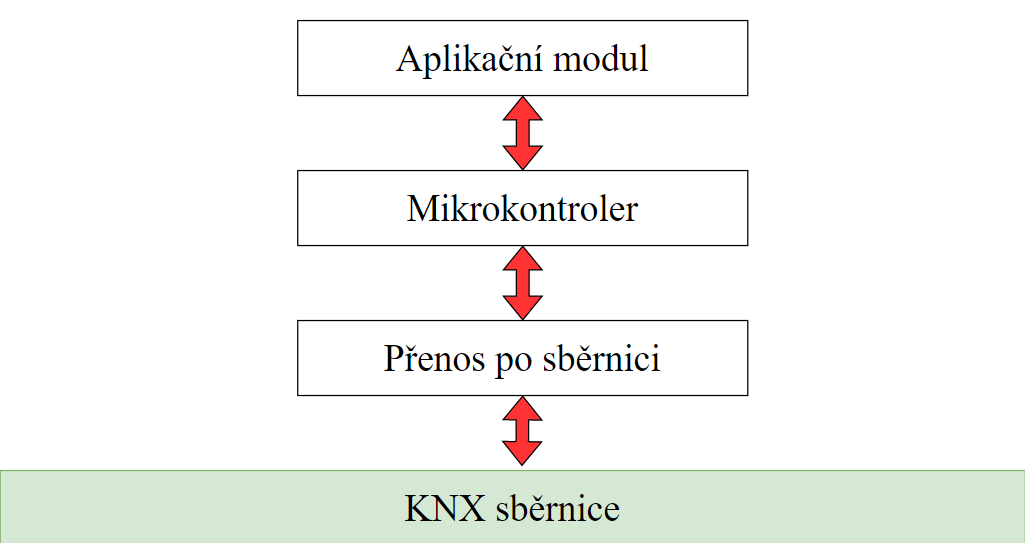
\includegraphics[scale=0.7]{obrazky/sbernice.png}
  \end{center}
  \caption[Součásti sběrnicového přístroje \cite{KNX principles}] {Součásti sběrnicového přístroje \cite{KNX principles}}
  \label{fig:Součásti sběrnicového přístroje}
\end{figure}
Přístroje lze ještě dělit na aktivní a pasivní. Pasivní přístroje nejsou součástí ICT, ale jedná se o podpůrné přístroje určené pro podporu procesu. Ve zkratce to znamená, že nekomunikují s ostatními přístroji. Jedním z příkladů pasivních přístrojů jsou napájecí zdroje.  Příkladem pasivních přístrojů jsou napájecí zdroje (Napájecí zdroje mohou být rozšířené ještě o ICT, ale není to časté).  
Aktivní přístroje lze rozdělit do těchto kategorií \cite{KNX principles}:
\begin{itemize}
\item Rozhraní - propojuje sběrnici a PC
\item Spojky - Optimalizují komunikaci v systému
\item Snímače - Předávají informace sběrnicovému systému
\item Akční členy - propojují klasické spotřebiče se sběrnicovým systémem
\end{itemize}

\subsection{Adresování}
\label{Adresování}
Individuální adresa je v instalaci jedinečná, tj. neexistuje další stejná adresa a požívá se k přesné identifikaci přístroje na sběrnici. Adresa je 16-bitová a je rozdělená na tři části (viz Obr. \ref{fig:Struktura individuální adresy]}).
\begin{figure}[!h]
  \begin{center}
    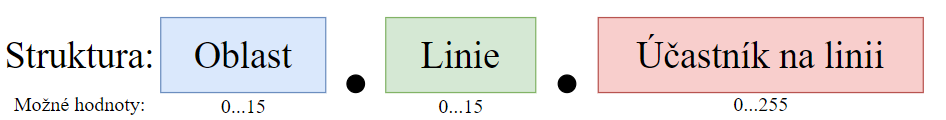
\includegraphics[scale=0.6]{obrazky/Adresovani.png}
  \end{center}
  \caption[Struktura individuální adresy \cite{Celkovy prehled)}]{Struktura individuální adresy \cite{Celkovy prehled}}
  \label{fig:Struktura individuální adresy]}
\end{figure}

Nastavování individuální adresy na přístroji probíhá většinou stiskem programovacího tlačítka na přístroji. Při stisknutí tlačítka se rozsvítí programovácí LED. Individuální adresa se přístroji přiděluje natrvalo. Po přidělení již ETS posílá příslušná data (aplikace, konfigurace, parametry, skupinové adresy).

Při uvedení do provozu komunikace probíhá pomocí skupinových adres. Jedná se o adresy definované programátorem pro každou funkci v systému. Celkově je možno použít 65535 adres s tím, že adresa 0/0/0 je rezervována pro tzv. broadcast (Hlášení všem přístrojům na sběrnici). Programátor si také může zvolit, kterou z uvedených struktur použije (viz Obr. \ref{fig:Příklad struktury skupinových adres}). 
\begin{figure}[!h]
  \begin{center}
    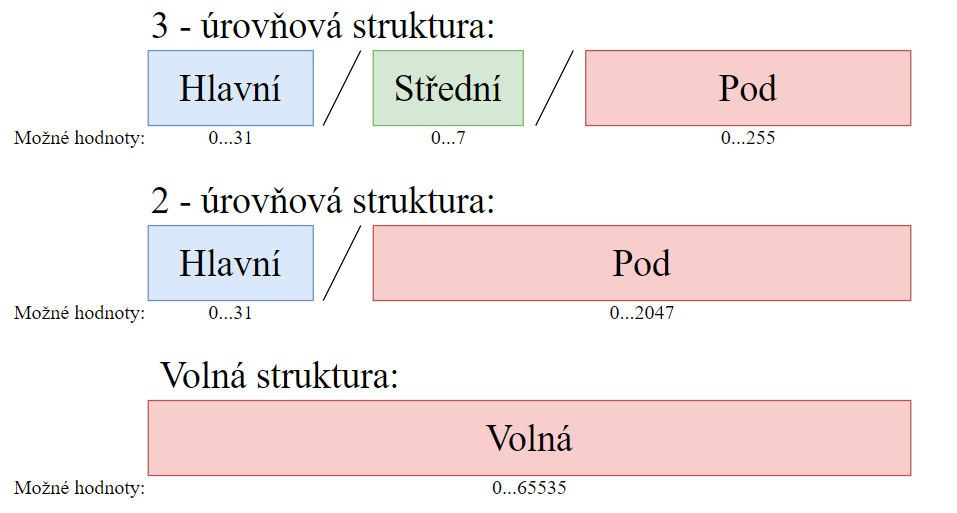
\includegraphics[scale=0.6]{obrazky/Skupinove adresovani.png}
  \end{center}
  \caption[Příklad struktury skupinových adres \cite{Celkovy prehled}]{Příklad struktury skupinových adres \cite{Celkovy prehled}}
  \label{fig:Příklad struktury skupinových adres}  
\end{figure}
Nejčastěji se využívá třístupňová struktura kvůli přehlednosti. Hlavní skupina se používá na číslo podlaží,  střední skupina na funkci (např. 1 = osvětlení, 2 = topení, 3 = stínění etc.)a podskupina pro konkrétní spotřebič, nebo skupinu spotřebičů. \cite{Celkovy prehled}
\\
\\
\\
\subsection{Komunikace po sběrnici}
Komunikace přístrojů na sběrnici probíhá pomocí tzv. telegramů (viz Obr. \ref{fig:Struktura telegramu}), kde je délka dat závislá na typu datového bodu  (1bit - 14bytů).
Nejdůležitější části telegramu jsou tři bloky \cite{Celkovy prehled}:
\begin{itemize}
\item Zdrojová adresa - udává adresu přístroje který telegram vyslal
\item Cílová adresa - adresa přístroje, kterému je telegram určen
\item Užitečná data - příkaz co má daný přístroj vykonat\\
\end{itemize}
\begin{figure}[!h]
  \begin{center}
    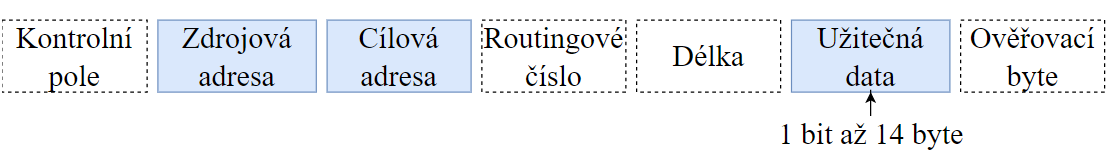
\includegraphics[scale=0.7]{obrazky/Struktura telegramu.png}
  \end{center}
  \caption[Struktura telegramu \cite{Celkovy prehled}]{Struktura telegramu \cite{Celkovy prehled}}
  \label{fig:Struktura telegramu}
\end{figure}
Telegramy na sběrnici čtou všechny přístroje, ale vykoná jej pouze přístroj určený cílovou adresou.

Komunikace na sběrnici probíhá pouze v případě, že je na sběrnici logická "1". V opačném případě je sběrnice přeplněná a pokračuje ve vysílá pouze přístroj s logickou "0" (viz Obr. \ref{fig:Struktura bitu kroucené dvojlinky}). \cite{Celkovy prehled}

\begin{figure}[!h]
  \begin{center}
    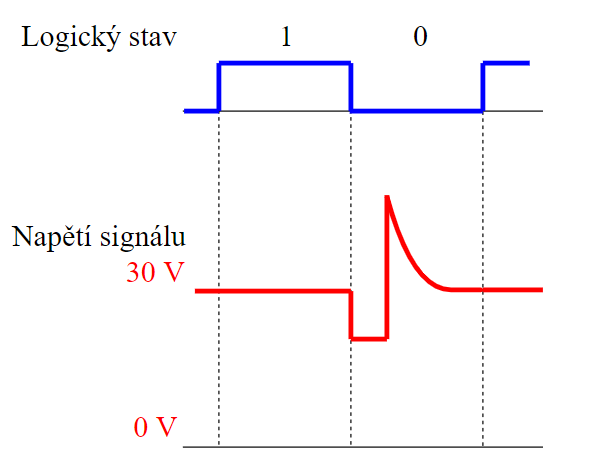
\includegraphics[scale=0.7]{obrazky/Struktura bitu.png}
  \end{center}
  \caption[Struktura bitu kroucené dvojlinky \cite{Celkovy prehled}]{Struktura bitu kroucené dvojlinky \cite{Celkovy prehled}}
  \label{fig:Struktura bitu kroucené dvojlinky}
\end{figure}

Aby jsme se vyhli kolizím a jeden z přístrojů mohl vysílat je přenos řízen principem CSMA/CA (Carrier Sense Multiple Access with Collision Avoidance vícenásobný přenos s vyhnutím se kolizím), který funguje tak, že pokud přístroj odesílající logickou “1” detekuje logickou “0”, aby se uvolnila cesta pro přenos jinému přístroji. Přístroj s přerušeným přenosem sleduje provoz na sběrnici a vyčká do konce přenosu jiného zařízení a poté zkusí znova vysílat. \cite{Celkovy prehled}
\subsection{KNXnet/IP}

Pro překlenutí fyzické sběrnice KNX a IP sítí slouží protokol \emph{KNXnet/IP}, který definuje dva základní režimy:

\subsubsection{Tunelování (Tunnelling)}  
Tunelování umožňuje bod–bod komunikaci mezi KNX sběrnicí a IP klientem. KNX telegramy se zabalí do UDP/IP paketů a posílají na port 3671. Server udržuje pro každé TCP/UDP spojení vlastní \textit{Individual Address}, kterou klientovi přidělí při navázání tunelu. Z toho v praxi vyplývají tyto tři možné režimy \cite{KNXTunnel}:

\begin{itemize}
  \item \textbf{Sdílená adresa (Shared IA)}  
    \newline Režim A používá KNXnet/IP Server \textbf{stejnou} \textit{Individual Address} pro všechny tunelovací relace. Klienti tedy sdílí mezi sebou jeden fyzický adresní bod na TP-lince. Výsledkem je jednoduchá konfigurace, ale horší rozlišovací schopnost mezi klienty posílajícími telegram.
  \item \textbf{Dedikovaná adresa (Dedicated IA)}  
    \newline Režim B přidělí každému tunelovacímu klientovi \textbf{unikátní} \textit{Individual Address}. Tudíž lze monitorovat a spravovat každou relaci individuálně.

  \item \textbf{Kombinovaný režim (Routing + Tunnelling)}  
    \newline V Režimu C server kromě přidělení dedikovaných tunelů funguje i jako KNX/IP Router pro multicast skupinových telegramů. Má tedy jednu IA pro routování (např. 1.1.0), tak další IA pro tunnelling relace. Díky tomu zvládne jak point-to-point servis a diagnostiku, tak i point-to-multipoint přenosy mezi subnety. \newline
\end{itemize}
\begin{figure}[!h]
  \begin{center}
    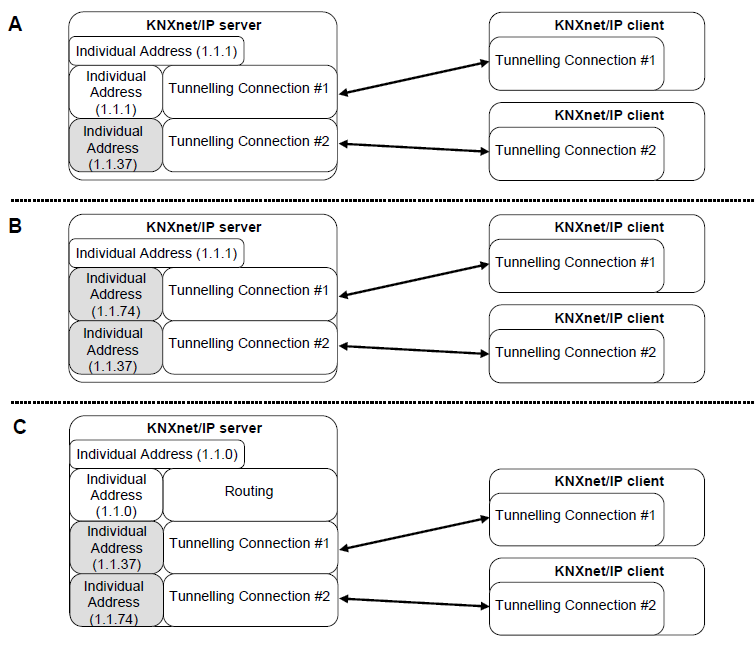
\includegraphics[scale=0.7]{obrazky/KNX_Tunelling.png}
  \end{center}
  \caption[Tunelování \cite{KNXTunnel}]{Tunelování \cite{KNXTunnel}}
  \label{fig:Tunelovani}
\end{figure}
\subsubsection{Routing (Routing)} 
Routing zajišťuje přenos skupinových (point-to-multipoint) telegramů mezi více KNX liniovými segmenty(linky/subnety). Každý KNXnet/IP Router přijímá příchozí telegramy na multicastové skupině a podle filtrovaných adres je znovu vysílá na KNX sběrnici. Díky tomu umožňuje velmi rychlé doručení telegramů současně do více destinací. \cite{KNXRouting}
\begin{figure}[!h]
  \begin{center}
    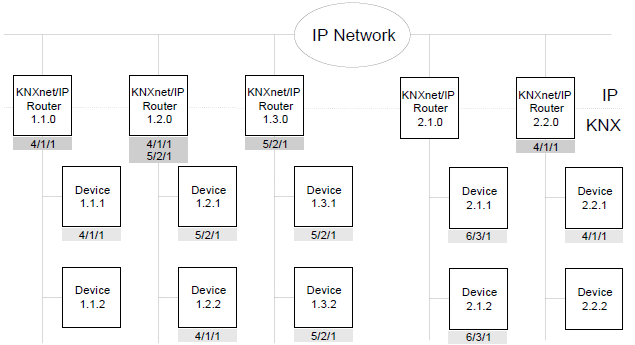
\includegraphics[scale=0.7]{obrazky/KNX_Routing.png}
  \end{center}
  \caption[Routování \cite{KNXRouting}]{Routování \cite{KNXRouting}}
  \label{fig:Routovani}
\end{figure}
\subsection{Datový bod}
Datové typy byly standardizovány za účelem zajištění kompatibility podobných přístrojů od různých výrobců. Jedná se například o stmívání, žaluzie a hodiny. Standardizace zahrnuje požadavky na formát dat a strukturu komunikačních objektů snímačů a akčních členů. I tak existuje více druhů datových bodů (DPT) se stejnou funkcionalitou. Kombinace různých typů DPT se nazývají funkčními bloky. \cite{Celkovy prehled}
\\Skutečná informace datového bodu:
\begin{itemize}
    \item Není uložena v paměti zařízení.
    \item Není nikdy součástí telegramu
    \item Je pouze v projektu ETS\\
\end{itemize}
Typy datových bodů jsou zvláště důležité pro diagnostiku to znamená, že umožňují ETS monitorovat data spojená se skupinovými objekty, např. místo "data = 85 A8" je zobrazeno "data = -6 °C". \cite{Datapoint}\\
\\Struktura datového bodu a notace \cite{Datapoint}:
\begin{itemize}
    \item Datový typ : formát + kódování
    \item Velikost: rozsah hodnot + jednotky
\end{itemize}
Notace datového bodu se píše ve tvaru X.YYY, neboli DATOVÝ TYP.VELIKOST.

\begin{table}[h]
 \caption[Přehled nejpoužívanějších datových typů]{Přehled nejpoužívanějších datových typů}
   \small
    \centering
	  \begin{tabular}{|c|c|c|}
	    \hline
	    Značení & Formát  & Funkce  \\
	    \hline\hline
	    1.yyy & boolean & přepínání (001), krok (007),... \\
	    \hline
	    3.yyy & boolean + 3-bit unsigned & stmívání \\
	    \hline
	    5.yyy & 8-bit unsigned + 3-bit unsigned & stmívání(0-100\%), pozice rolet(0-100\%)\\
	    \hline
	    7.yyy & boolean + 3-bit unsigned & čitač pulsů \\
	    \hline
	    9.yyy & 16-bit float & přenos hodnoty teploty, jasu, rychlost větru \\
	    \hline
	    14.yyy & 32-bit float & nastavení teploty\\
	    \hline
	    19.yyy & čas + data & výstupy obrazovek \\
	    \hline
	    20.yyy & 8-bit enumerace & Topení, chlazení a ventilace ('komfort',...) \\
	    \hline
	  \end{tabular}
\end{table}

Díky existenci datového bodu jsme schopní nastavit hodnotu osvětlení 3 různými způsoby \cite{Systemove Argumenty}:
\begin{itemize}
    \item Zapnutí/Vypnutí
    \item Krokové stmívání - Při poslání telegramu "start stmívání" osvětlení krokově roste o definovanou hodnotu. Po poslání "stop stmívání" hodnota neroste.
    \item Procentuální stmívání- Realizuje se pomocí cyklického posílání telegramu. Při každém přijetí telegramu se zvedne jas o nastavenou hodnotu.
\end{itemize}

\section{Zabezpečení}
Rozdíl mezi zařízeními KNX a zabezpečenými KNX Secure je ten, že zařízení KNX Secure jsou schopna šifrovat a dešifrovat telegramy. Tato technologie dodává instalaci extra zabezpečení, a to během uvádění instalace do provozu, tak i poté za běhu. Telegramy jsou zašifrované zabezpečenými zařízeními KNX se nazývají zabezpečené telegramy.
\\Lze rozlišit dva typy šifrovaných telegramů KNX \cite{KNX Secure}:
\begin{itemize}
\item{Zcela zašifrované}
\begin{itemize}
\item{Lze použít pouze na zařízeních KNX IP a je označováno jako KNX IP Secure.}
\item{Používá se, pro zabezpečení části intalace, která je vystavená externí IP síti (typicky se jedná o páteřní linku).}
\end{itemize}
\item{Čatečně zašifrované}
\begin{itemize}
\item{Lze požít na libovolné komunikační zařízní KNX. Zařízení používající tento typ zabezpečení se nazývají KNX Data Secure}
\item{Toto šifrování můžeme použít i pro KNX IP, ale pouze pro tu část instalace, která není vystavena externí IP síti.}
\end{itemize}
\end{itemize}
Oba typy zabezpečení obsahují MAC (Message Authentication Code).
\\Zabezpečená zařízení mají zabezpečený režim, který je v projektu ETS reprezentován vlastností nazvanou „Secure Commissioning“. Pouze když je tento režim aktivován, zařízení je schopno šifrovat a dešifrovat telegramy.

Zabezpečená zařízení mají tzv. "Tool Key". V moment, když je aktivován zabezpečený režim zařízení, je ETS schopen komunikovat s tímto zařízením pouze pokud zná Tool Key tohoto zařízení.

Zabezpečená zařízení obsahují také Factory Default Setup Key (FDSK). FDSK je jedinečný pro každé zařízení a nelze jej upravovat ani mazat. ETS tento klíč může načíst jenom pomocí certifikátu (25znakový kód, který obsahuje sériové číslo a FDSK). Tool Key je v zásadě z výroby nastaven na FDSK. Tool Key může být také zpětně nastaven na FDSK pomocí tzv. "master resetu", který uvadí výrobce. 

Po přidání zabezpečeného zařízení KNX  do ETS a po přidání jeho certifikátu, ETS automaticky nastaví svůj Tool Key v projektu. To znamená, že uživatel ETS nemůže definovat/upravit Tool Key ručně, Tool Key také není viditelný pro uživatele ETS. \cite{KNX Secure}

\section{Topologie}
Základním kamenem topologie je hlavní linie, na kterou lze připojit až 256 přístrojů (účastníků sběrnice - US). Tato linie lze rozdělit až na 15 dalších segmentů za použití liniových opakovačů/spojek (LS). Na takto vzniklé segmenty (linie) připojit dalších 256 US. To vše ovšem závisí také na spotřebě přístrojů použitých v instalaci. To znamená, že celková spotřeba všech přístrojů nesmí překročit jmenovitý proud na druhé straně sběrnicového zdroje, který každá linie musí mít vlastní. Také lze mít maximálně 4 000 US na celé topologii. Toto množství lze také navýšit za použití oblastní spojky (OS) díky na páteřní linii. Po připojení vznikne tzv. nadřazená páteřní linie, která může pojmout až 16 oblastních spojek a celek rozdělí na dílčí páteřní linie. Celkový počet US na takovéto linii může být až 61 000. Reálné množství je v tomto případě omezeno zdrojem s tlumivkou (NZ/TI). \cite{Topologie}\\\\
Pro sběrnici KNX lze použít pouze tyto struktury kabeláže:
\begin{itemize}
    \item Hvězdicová
     \item Liniová
     \item Stromová
     \item Kombinace výše uvedených\\ \\ \\
\end{itemize}
\begin{figure}[!h]
  \begin{center}
    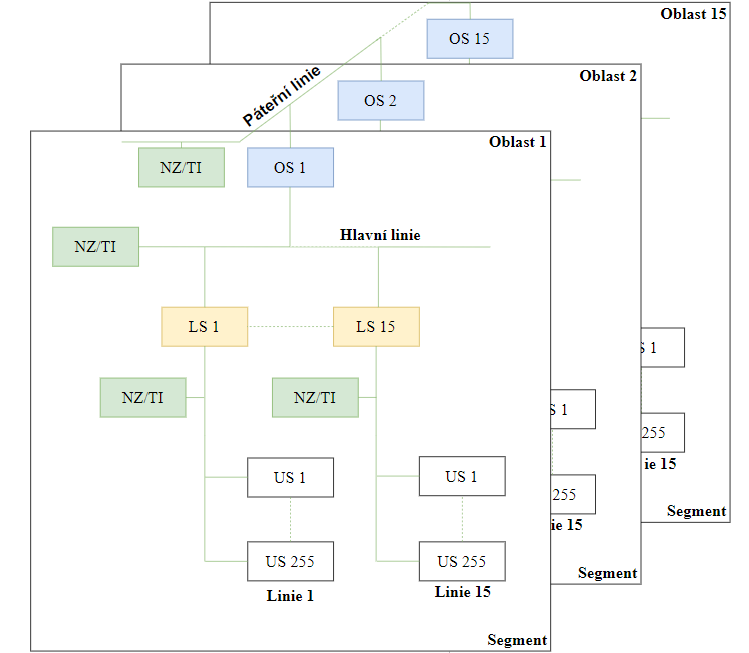
\includegraphics[scale=0.6]{obrazky/Ukazka topologie.png}
  \end{center}
  \caption[Ukázka topologie KNX\cite{Topologie}]{Ukázka topologie KNX\cite{Topologie}}
  \label{fig:Ukázka topologie KNX}
\end{figure}

\newpage
\subsection{Individuální adresa}
Individuální adresa se nastavuje s ohledem na umístění v topologii (Viz. Podkapitola \ref{Adresování}).
\begin{table}[h]
 \caption[Individuální adresy v topologii \cite{Topologie}]{Individuální adresy v topologii \cite{Topologie}}
   \small
    \centering
	  \begin{tabular}{|c|c|c|}
	    \hline
	    Prvek & Adresa & Funkce  \\
	    \hline\hline
	    Oblast & 0 & adresuje účastníky v páteřní linii \\
	    \hline
	    Oblast & 1...15 & adresuje oblasti \\
	    \hline
	    Linie & 0 & adresuje hlavní linii příslušné oblasti \\
	    \hline
	    Linie & 1...15 & adresuje linie obsažené v oblasti\\ 
	    \hline
	    Účastník na sběrnici & 0 & adresuje liniovou spojku příslušné linie \\
	    \hline
	    Účastník na sběrnici & 1...255 & adresuje sběrnicové přístroje obsažené v linii \\
	    \hline
	  \end{tabular}
\end{table}
\newpage
\subsection{Spojka}
V případě,že jsou v instalaci použity spojky a mají přiřazeny správné individuální adresy, budou při projektování v programu ETS (Kapitola \ref{ETS}) automaticky vytvořeny filtrační tabulky jednotlivých spojek. Filtrační tabulka obsahuje skupinové adresy, které smí projít skrz příslušnou spojku (obsahuje všechny obsažené skupinové adresy, které adresují SU umístěné za spojkou). Tudíž každá linie pracuje nezávisle.

 Spojky jsou vytvořeny pro montáž na DIN lištu, kde se připojují primární i sekundární linie pomocí sběrnicové svorkovnice. Primární linie také funguje, jako napájení mikrokontroleru a při výpadku sítě ohlásí tuto skutečnost na sekundární linii. Jednou z výhod pojky je možnost programování z obou linií. Obsahují také žluté signalizující LED, které blikají pouze v případě, že spojka propustí telegram na příslušnou linii. Další vlastností spojky je galvanické oddělení mezi primární a sekundární linií. Poslední vlastností spojky je možnost přeměny na liniový opakovač. Opakovač se rozliší od spojky absencí nuly na konci individuální adresy (X.X.1 apod.). Využívá se pro rozšíření linie o další segment s 64 US. Tento úsek je limitován délkou kabelu, který může měřit maximálně 1000m. \cite{Topologie}
 
\subsection{Routingové číslo}
Každý telegram, který je vyslán přístrojem na obsahuje routingové číslo, které začíná na hodnotě 6. Toto číslo při každém průchodu spojkou, či opakovačem se dekrementuje dokud nedosáhne nulové hodnoty. Tuto vlastnost berou filtrační tabulky v potaz.
Pokud se jedná o servisní telegram, tak routingové číslo má hodnotu 7, která se při průchodu spojkou nedekrementuje. \footnote{Spojky vyrobeny po roce 2019 mají schopnost tuto hodnotu dekrementovat}. Tuto skutečnost berou v potaz i filtrační tabulky, které toto číslo ignorují, a tudíž všechny spojky tento telegram propustí. Tento telegram se vždy dostane k požadovanému účastníku bez ohledu na umístění.
Toto číslo také brání zasmyčkování (nekonečnému kolování) telegramu. \cite{Topologie}
\subsection{Interní a externí rozhraní}
Systém KNX je otevřený jiným systémům za použití vhodných rozhraní umístěných na libovolné linii (většinou se jedná o páteřní linii). Lze připojit například programovatelný logický automat (PLC), digitální síť integrovaných služeb (ISDN), systémová technika budov, internet a mnohé další.
Tato rozhraní přenáší obousměrně zprávy, které převede na komunikační protokol.

Nejedná se ovšem jenom o spojovaní KNX s externími médii, ale je možno spojit různá KNX média mezi sebou (např. spojení TP, RF, optika) \cite{Topologie}.